\section{Distributed Bragg reflector}

The first genuine multilayer benchmark is a quarter-wave distributed
Bragg reflector (DBR). The stack alternates a high-index and a low-index
quarter-wave layer and is repeated $N$ times on a glass substrate. The
materials are TiO$_2$ ($n_H = 2.35$) and SiO$_2$ ($n_L = 1.38$) on glass
($n_s = 1.52$) in air ($n_0 = 1.00$), with the design wavelength fixed at
$\lambda_0 = \SI{550}{\nano\metre}$. Each layer thickness equals one
optical quarter-wavelength, so
$d_H = \lambda_0/(4 n_H) \approx \SI{58.5}{\nano\metre}$ and
$d_L = \lambda_0/(4 n_L) \approx \SI{99.6}{\nano\metre}$. The refractive
index list fed to the TMM is
\[
  (n_0,\ n_H,\ n_L,\ n_H,\ n_L,\ \ldots,\ n_H,\ n_L,\ n_s),
\]
with the $(n_H, n_L)$ block repeated $N$ times, and the thickness list is
the corresponding $(d_H, d_L)^{N}$ sequence.

Two analytical results frame the behaviour. The width of the high-reflectance
stopband centred at $\lambda_0$ is
\begin{equation}
  \frac{\Delta\lambda}{\lambda_0} = \frac{4}{\pi}\arcsin\!\left(\frac{n_H - n_L}{n_H + n_L}\right), \label{eq:dbr-band}
\end{equation}
and the peak reflectance at $\lambda_0$, with the effective substrate
admittance $Y_{\rm eff} = (n_H/n_L)^{2N}\,n_s$ for the stack terminated in
$n_L$\,/\,substrate, is
\begin{equation}
  R_{\rm peak} = \left(\frac{n_0 - Y_{\rm eff}}{n_0 + Y_{\rm eff}}\right)^{2}. \label{eq:dbr-Rpeak}
\end{equation}
Panel (a) plots $R(\lambda)$ across \SIrange{400}{800}{\nano\metre} for
$N = 2, 5, 10$ pairs with the stopband from~\eqref{eq:dbr-band} shaded.
Panel (b) sweeps $N$ from $1$ to $15$ and compares the TMM peak reflectance
at $\lambda_0$ with~\eqref{eq:dbr-Rpeak}.

\begin{center}
\begin{tikzpicture}
  \fill[black!4] (0, 0) rectangle (5, 1.2);
  \foreach \i in {0,...,3} {
    \fill[blue!20]  (0,{-0.22*(2*\i+1)}) rectangle (5, {-0.22*(2*\i)});
    \fill[green!20] (0,{-0.22*(2*\i+2)}) rectangle (5, {-0.22*(2*\i+1)});
  }
  \fill[blue!6] (0,-2.2) rectangle (5,-1.8);
  \draw[thick] (0,0) -- (5,0);
  \draw[thick] (0,-1.8) -- (5,-1.8);
  \node[lbl, anchor=east] at (4.9, 0.8) {air};
  \node[lbl, anchor=east] at (4.9,-0.9) {$(n_H n_L)^N$};
  \node[lbl, anchor=east] at (4.9,-2.0) {glass};
  \raysketch{1.6}{0}{f}
\end{tikzpicture}
\end{center}

\begin{figure}[!htbp]
  \centering
  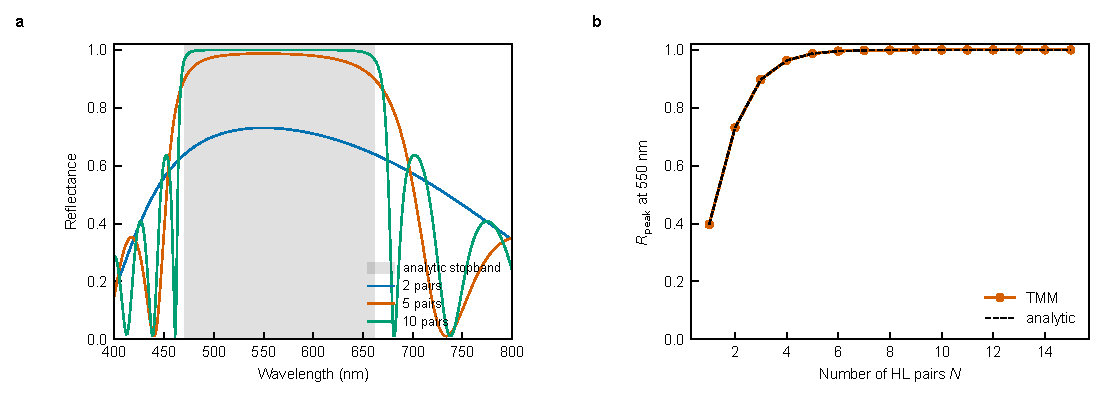
\includegraphics[width=\textwidth]{10_bragg_mirror.pdf}
  \caption{(a) Reflectance of the DBR for $N = 2, 5, 10$ pairs on glass; the shaded band marks the analytic stopband~\eqref{eq:dbr-band}. (b) Peak reflectance at $\lambda_0$ against the admittance formula~\eqref{eq:dbr-Rpeak}.}
  \label{fig:bragg}
\end{figure}

The TMM peak reflectance tracks the admittance formula~\eqref{eq:dbr-Rpeak}
over $N = 1\ldots 15$ with
$|\Delta R_{\rm peak}| \approx \num{1e-15}$, and the high-reflectance
window in panel (a) falls inside the analytic stopband at all pair counts.
For $N \gtrsim 10$ the reflectance saturates above $99.99\%$ at the design
wavelength, and the stopband edges become progressively sharper with
increasing $N$; outside the stopband the curves show the usual ripple from
the finite number of periods, which the TMM reproduces in amplitude and
phase.


